% ======================================================================
\section{Experiments: Selective Hamiltonian Risk Adaptation}
\label{sec:experiments}
% ======================================================================

The experiments test one question across increasingly difficult settings:
\emph{does Hamiltonian context enrichment produce selective adaptation ---
activating risk forces when a safer feasible alternative exists and
suppressing them when it does not?}
Static RELLIS tests this spatially in real off-road semantic maps.
RELLIS-Dyn tests it temporally when the map changes during execution,
isolating three contributions via paired ablations.
DFC2018 tests whether enrichment repairs a static geometry-only scaffold.
Highway-env tests the same activation/suppression split for interaction
risk in traffic.

% ----------------------------------------------------------------------
\subsection{Experimental Questions}
\label{sec:exp_questions}
% ----------------------------------------------------------------------

Seven questions organize the evaluation.
\textbf{RQ1 (spatial activation):} does context-enriched field activate the context
force toward a feasible lower-risk direction when one exists?
\textbf{RQ2 (spatial suppression):} does context-enriched field suppress the force
when a lower-risk-looking direction is blocked?
\textbf{RQ3 (temporal activation):} does context-enriched field activate before a
replanning baseline when material risk changes mid-trajectory?
\textbf{RQ4 (temporal suppression):} does context-enriched field avoid pursuing an
escape that has closed or not yet opened?
\textbf{RQ5 (within-episode selectivity):} can the same rollout
suppress force before an escape exists \emph{and} activate immediately
after?
\textbf{RQ6 (force channel vs.\ loss reweighting):} must risk enter the
Hamiltonian force channel, or is adding it to the training loss
sufficient?
\textbf{RQ7 (tail risk):} does tail-risk training reduce severe and
persistent violations, not only mean risk?

% ----------------------------------------------------------------------
\subsection{Domains, Regimes, and Events}
\label{sec:exp_domains}
% ----------------------------------------------------------------------

All domains share three regimes.
\textbf{R1}: a feasible lower-risk alternative exists.
\textbf{R2}: a lower-risk-looking alternative is blocked, outside the
traversable mask, or dynamically unsafe.
\textbf{R3}: the context is risk-neutral; context-enriched field should preserve the
geometry scaffold.

In RELLIS-3D, semantic labels project into a local BEV soft-risk field
$r(x,y)\in[0,1]$ and hard-hazard signed-distance field $\phi(x,y)$.
RELLIS-Dyn extends the R1/R2 decomposition from space to time by
injecting one of eight events at $t_{\rm event}$: soft-risk gradient
events (\emph{mud onset}, \emph{puddle expansion}); hard-boundary events
(\emph{corridor closes}, \emph{corridor opens}); dynamic-obstacle events
(\emph{crossing obstacle}, \emph{moving obstacle blocks detour}); and
compound/delayed events (\emph{mud onset with blocked detour},
\emph{delayed escape opens}).
For the within-episode benchmark we additionally use
\emph{delayed required escape}: the escape is blocked before
$t_{\rm escape}$; when it opens the original scaffold becomes unsafe.
Full event definitions and the eight-event breakdown are in
Appendix~\ref{app:rellis_dyn_details}.

% ----------------------------------------------------------------------
\subsection{Mechanistic Metrics}
\label{sec:exp_mechanistic_metrics}
% ----------------------------------------------------------------------

Let $F_{\mathrm{ctx}}=-\nabla_q H_{\mathrm{ctx}}$, $d_{\mathrm{scaf}}$
the geometry scaffold direction, and $d_{\mathrm{safe}}$ the lowest-risk
feasible direction when it improves over $d_{\mathrm{scaf}}$ by a margin.
Spatial selectivity uses
\begin{equation}
\mathrm{CAR}=\Pr[\langle F_{\mathrm{ctx}},d_{\mathrm{safe}}\rangle{>}\epsilon\mid R1],\quad
\mathrm{FAR}=\Pr[|P_\perp F_{\mathrm{ctx}}|{>}\epsilon\mid R2],\quad
\mathrm{SR}=\frac{\mathbb{E}[|P_\perp F_{\mathrm{ctx}}|\mid R1]}
               {\mathbb{E}[|P_\perp F_{\mathrm{ctx}}|\mid R2]},
\end{equation}
and AUPRC of activation predicting R1 (threshold-independent).
Temporal metrics: \emph{reaction delay} (first step after $t_{\rm event}$
where lateral displacement from the pre-event scaffold exceeds $\delta$);
\emph{stale exposure} (violation accumulated before reaction);
\emph{false pre-activation} (fraction of delayed-escape episodes where
lateral force exceeds $\epsilon$ before $t_{\rm escape}$);
\emph{suppress rate} ($1 -$ false pre-activation);
\emph{opportunity-normalized delay} (reaction delay divided by the
available reaction window $T - t_{\rm escape}$).
Post-event violation CVaR (hard contact weighted separately from soft
exposure) is the primary tail metric;
Appendix Table~\ref{tab:app_rellis_dyn_delay_sensitivity} shows
stability across $\delta$.

% ----------------------------------------------------------------------
\subsection{RELLIS-3D: Spatial Selectivity}
\label{sec:exp_rellis_static}
% ----------------------------------------------------------------------

RELLIS static answers RQ1 and RQ2 on 2{,}250 BEV episodes across five
sequences evaluated with leave-one-sequence-out splits.
Table~\ref{tab:rellis_selectivity} reports six variants sorted by SR;
confidence intervals are in Appendix Table~\ref{tab:app_rellis_full}.

\begin{table}[t]
\centering
\caption{\textbf{RELLIS-3D spatial selectivity.}
CAR measures activation frequency in R1; SR measures whether force
concentrates in R1 over R2.
Black-box CVaR achieves the highest CAR but SR~$1.292$---it fires
nearly as strongly in blocked regimes as in feasible ones.
The route-aware context-enriched field leads on SR and AUPRC, indicating selective rather
than uniform activation.
fixed-coeff context field confirms that context-conditioned coefficients
are essential: without them FAR reaches $0.888$.}
\label{tab:rellis_selectivity}
\small
\setlength{\tabcolsep}{5pt}
\renewcommand{\arraystretch}{1.1}
\begin{tabular}{lcccc}
\toprule
Method & CAR$\uparrow$ & FAR$\downarrow$ & SR$\uparrow$ & AUPRC$\uparrow$ \\
\midrule
Geom. scaffold          & $0.000$ & $0.000$ & $0.000$ & $0.000$ \\
Scalar context field            & $0.378$ & $0.752$ & $1.031$ & $0.008$ \\
Fixed-coeff context field    & $0.566$ & $0.888$ & $1.123$ & $0.008$ \\
Non-route directional Ctx  & $0.135$ & $0.178$ & $1.165$ & $0.206$ \\
Black-box CVaR policy     & $0.884$ & $0.129$ & $1.292$ & $0.206$ \\
\textbf{Route-aware Ctx} & $\mathbf{0.837}$ & $\mathbf{0.114}$
                           & $\mathbf{2.358}$ & $\mathbf{0.289}$ \\
\bottomrule
\end{tabular}
\end{table}

scalar context field fires too often in R2 (FAR~$0.752$). Non-route
directional force suppresses false activation but misses most R1
opportunities (CAR~$0.135$). Black-box CVaR, which uses the same
local BEV patch under the same CVaR objective but no Hamiltonian
structure, achieves the highest raw CAR yet SR only~$1.292$: it learns
to follow risk gradients but applies comparable force whether or not a
feasible escape exists. route-aware context-enriched field achieves SR~$2.358$ and
AUPRC~$0.289$ because the route-aware gate suppresses the soft-risk
force when no locally feasible lower-risk candidate exists.
fixed-coeff context field (fixed $\lambda_s,\lambda_h$) reaches
FAR~$0.888$, confirming that context-conditioned coefficient prediction
is necessary for suppression.
The spatial result anticipates the temporal one: Section~\ref{sec:exp_rellis_dyn}
shows black-box CVaR's uniform activation produces $0.920$ false
pre-activation and $0.200$ navigation success on the delayed-escape
benchmark.

% ----------------------------------------------------------------------
\subsection{RELLIS-Dyn: Temporal Selectivity}
\label{sec:exp_rellis_dyn}
% ----------------------------------------------------------------------

RELLIS-Dyn asks whether the context force activates at the right
\emph{time}, not only in the right direction.
All methods receive the same updated BEV patch at every step; the only
difference is how they use it.
The context-enriched field updates its Hamiltonian force directly from the new patch;
local planners replan explicitly; reactive baselines use a one-step
control rule.

\paragraph{Delayed-required-escape: the primary temporal benchmark.}

The delayed-required-escape event is the main head-to-head RELLIS-Dyn
benchmark because it requires both parts of the selectivity signature in
one rollout.
Before $t_{\rm escape}$ the escape is blocked (R2 behavior required);
at $t_{\rm escape}$ it opens and the original scaffold becomes
unsafe (R1 behavior required).
Correct temporal selectivity means suppressing force throughout the
blocked window and activating immediately after.
Table~\ref{tab:delayed_escape} reports the head-to-head comparison
against reactive and sampling-based local baselines, then isolates the
three contributions of route-aware context-enriched field.

\begin{table}[t]
\centering
\caption{\textbf{Delayed-required-escape temporal benchmark} (100 episodes).
The escape is blocked before $t_{\rm escape}$ (R2 required) and
opens thereafter with the original scaffold becoming unsafe (R1
required).
Three paired comparisons isolate three contributions:
\emph{Hamiltonian structure} (black-box CVaR vs.\ Route-aware Ctx CVaR);
\emph{CVaR training} (expected-cost Ctx vs.\ Route-aware Ctx CVaR);
\emph{context-conditioning} (fixed coefficients vs.\ Route-aware Ctx CVaR).
$^\dagger$Violation CVaR below $0.51$ with success below $0.21$
reflects low violation by not navigating: these methods rarely enter the risky
region because they are stuck, not because they navigate safely.
Paired bootstrap $95\%$ CIs in
Appendix Table~\ref{tab:app_delayed_escape_ci}.}
\label{tab:delayed_escape}
\small
\setlength{\tabcolsep}{4pt}
\renewcommand{\arraystretch}{1.1}
\begin{tabular}{lcccc}
\toprule
Method
  & False pre-act$\downarrow$ & Suppress$\uparrow$
  & Success$\uparrow$ & Viol.\ CVaR$\downarrow$ \\
\midrule
Geom. scaffold        & $0.000$ & $1.000$ & $0.030$ & $1.894$ \\
Risk-loss-only          & $0.420$ & $0.580$ & $0.040$ & $1.793$ \\
\midrule
Fixed-coeff context field     & $0.990$ & $0.010$ & $0.030$ & $0.463^\dagger$ \\
Black-box CVaR policy   & $0.920$ & $0.080$ & $0.200$ & $0.503^\dagger$ \\
DWA semantic            & $0.950$ & $0.050$ & $0.480$ & $0.695$ \\
MPPI semantic           & $0.950$ & $0.050$ & $0.240$ & $0.831$ \\
Ctx-enriched, expected cost  & $0.370$ & $0.630$ & $0.620$ & $0.855$ \\
\textbf{Route-aware Ctx CVaR}
  & $\mathbf{0.180}$ & $\mathbf{0.820}$
  & $\mathbf{0.810}$ & $\mathbf{0.740}$ \\
\bottomrule
\end{tabular}
\end{table}

\begin{figure*}[t]
\centering
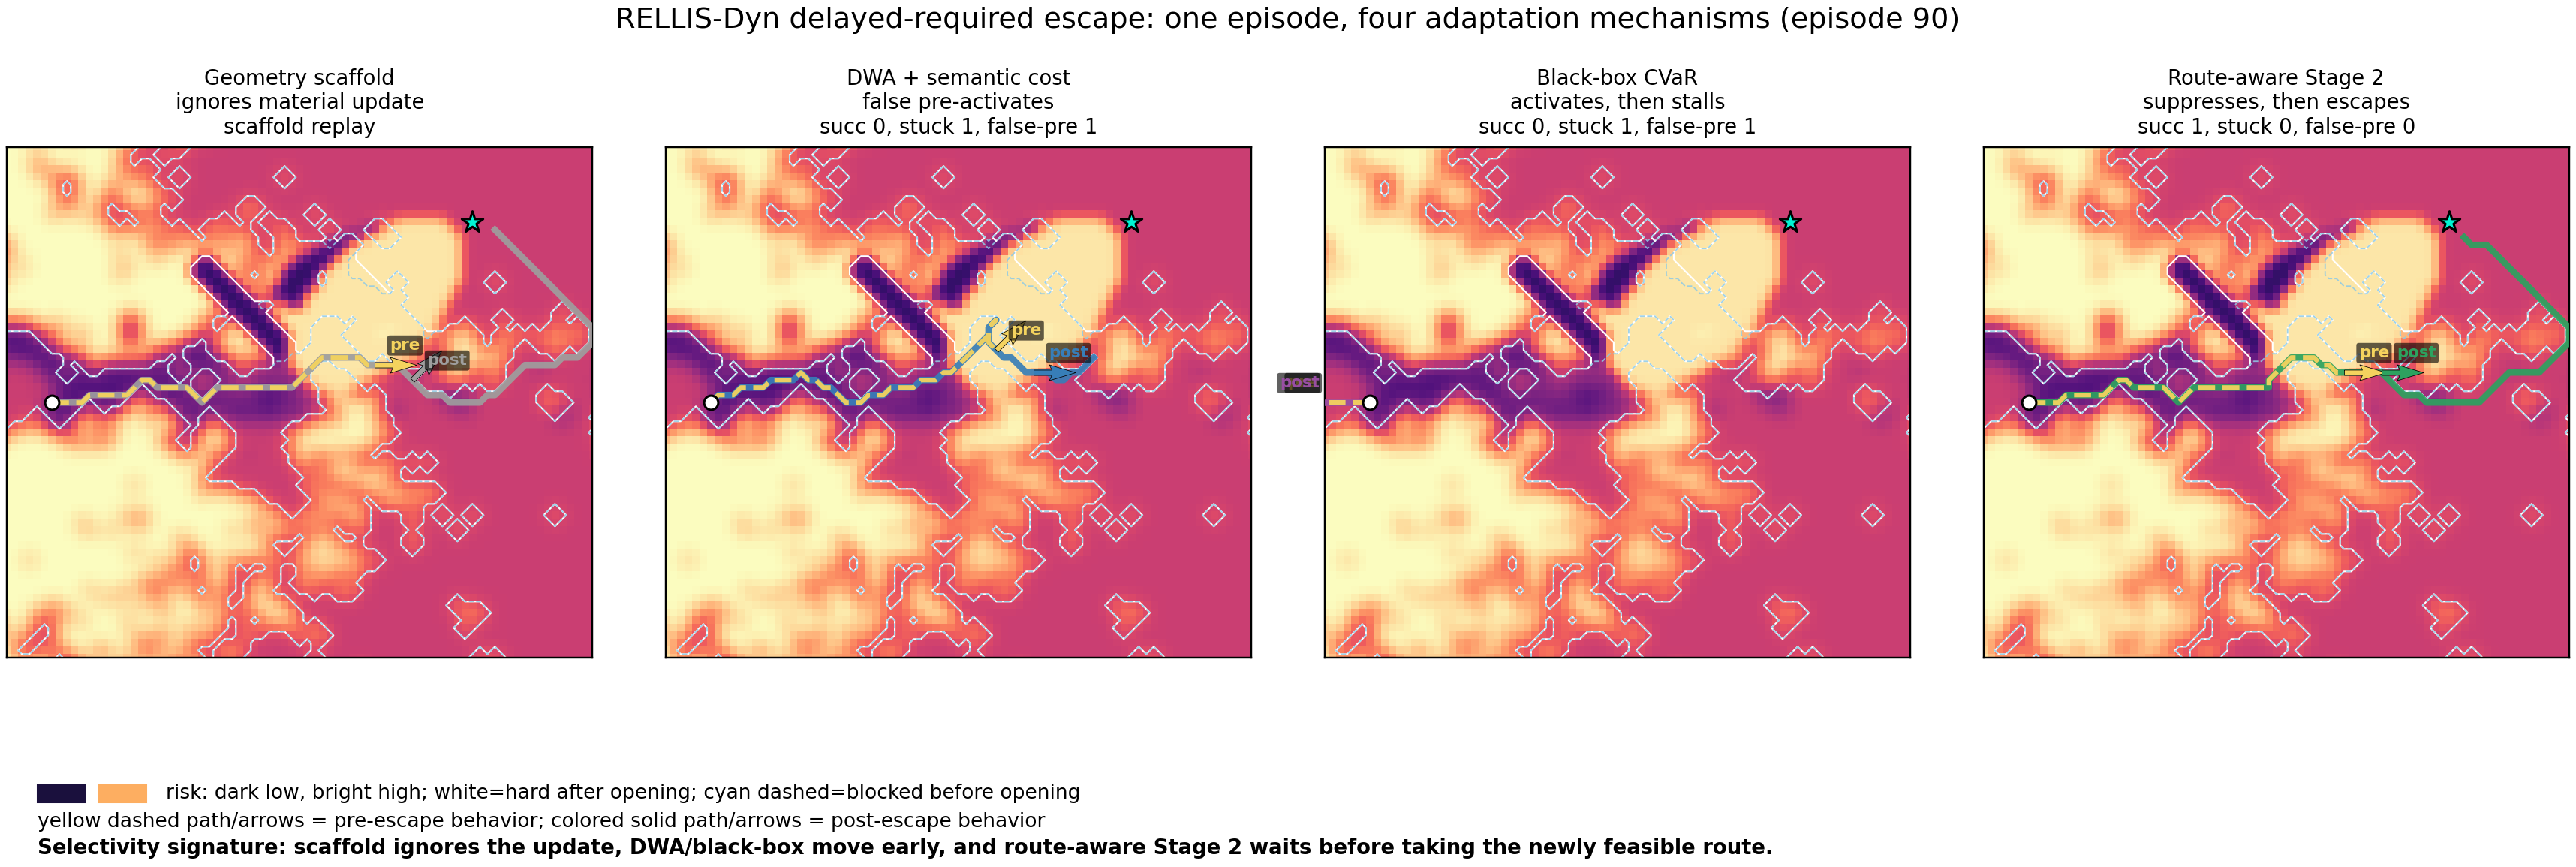
\includegraphics[width=\textwidth]{figures/rellis_dyn_spotlight_four_methods.png}
\caption{\textbf{Qualitative temporal selectivity in one delayed-required
escape episode.} The same RELLIS-Dyn BEV patch is executed by four methods.
Yellow dashed trajectories and arrows show behavior before the escape is
available; solid colored trajectories and arrows show behavior after it opens.
The geometry scaffold ignores the material update, DWA and the black-box CVaR
policy move before the escape is feasible and then stall, while route-aware
context enrichment suppresses the lateral force before $t_{\rm escape}$ and
takes the newly feasible route after it opens.}
\label{fig:rellis_dyn_spotlight}
\end{figure*}

\textbf{Head-to-head result.}
Route-aware Ctx CVaR is the only zero-replan method in
Table~\ref{tab:delayed_escape} that both suppresses premature escape attempts
and reliably reaches the goal: false pre-activation is $0.180$ versus
$0.950$ for DWA and semantic MPPI, while success is $0.810$ versus
$0.480$ and $0.240$.
This is the domain where the selectivity mechanism matters most: the right
action is to do nothing while the escape is blocked, then move immediately
once the local BEV patch makes the route feasible.

\textbf{Hamiltonian structure} (black-box CVaR vs.\ route-aware CVaR).
Both use the same CVaR objective and the same local BEV patch.
Black-box CVaR false pre-activation is $0.920$---it fires before the
escape exists on nearly every episode despite achieving static
CAR~$0.884$ in Table~\ref{tab:rellis_selectivity}.
Navigation success collapses to $0.200$.
The Hamiltonian force channel is not interchangeable with a learned
policy over the same inputs: the structured gradient update enables
temporal suppression that the black-box cannot replicate.

\textbf{CVaR training} (expected cost vs.\ route-aware CVaR).
Same architecture, same gate, different objective.
CVaR halves false pre-activation ($0.370\to0.180$), raises suppression
($0.630\to0.820$), improves navigation success by $30\%$
($0.620\to0.810$), and reduces violation CVaR ($0.855\to0.740$).
The R1-only subset (Appendix Table~\ref{tab:app_r1_only}) confirms that
CVaR reduces premature activation even when an escape genuinely
exists.
CVaR routes gradient through the tail rollouts where the force channel
must activate at the right time, not just in the right direction.

\textbf{Context-conditioning} (fixed-coeff vs.\ route-aware CVaR).
Same architecture, same objective, fixed $\lambda_s{=}\lambda_h$ vs.\
CNN-predicted.
Fixed-coeff false pre-activation is $0.990$, success $0.030$.
Without context-conditioned coefficients the method suppresses nothing
and navigates almost never.

\paragraph{Material-event aggregate.}
Table~\ref{tab:rellis_dyn_agg} reports the three-event material
subset (mud onset, corridor closes, corridor opens) for all methods
at $100$ episodes per event.
Moving-obstacle events are reported separately in
Appendix Table~\ref{tab:app_rellis_dyn_8event_groups} because DWA is
architecturally well-matched to reactive collision avoidance there.

\begin{table}[t]
\centering
\caption{\textbf{RELLIS-Dyn 3-event material aggregate} (100 episodes per
event, mud onset / corridor closes / corridor opens).
Soft-material CVaR is reported throughout; violation CVaR for the
ablation variants appears in Table~\ref{tab:delayed_escape}.
DWA success $0.567$ reflects stuck episodes (stuck rate $0.43$) that
accumulate low soft CVaR by not progressing through risky terrain.
Fixed-coeff and black-box CVaR low success reflects navigation failure,
not safety.
``No global search'' means no graph search or trajectory optimisation
at execution time; the gate in Route-aware Ctx samples $K{=}8$ local
primitives inside the same BEV window available to all methods.
$^\dagger$Oracle replanner uses global map access and is a privileged
reference ceiling.}
\label{tab:rellis_dyn_agg}
\small
\setlength{\tabcolsep}{3pt}
\renewcommand{\arraystretch}{1.1}
\resizebox{\linewidth}{!}{%
\begin{tabular}{llccccccc}
\toprule
Method & Family
  & Succ.$\uparrow$ & Soft CVaR$\downarrow$
  & Delay$\downarrow$ & Stuck$\downarrow$
  & Replans$\downarrow$ & ms/step$\downarrow$ \\
\midrule
Geom. scaffold   & scaffold
  & $1.000$ & $0.712$ & $16.2$ & $0.04$ & $0$ & $0.8$ \\
Risk-loss-only     & learned loss
  & $1.000$ & $0.673$ & $13.4$ & $0.03$ & $0$ & $0.9$ \\
\midrule
Fixed-coeff Ctx     & learned field
  & $0.120$ & $0.459$ & $1.47$ & $0.74$ & $0$ & $1.4$ \\
Black-box CVaR     & learned field
  & $0.273$ & $0.482$ & $3.61$ & $0.61$ & $0$ & $4.2$ \\
Ctx-enriched, exp.\ cost& learned field
  & $0.983$ & $0.465$ & $1.30$ & $0.02$ & $0$ & $2.1$ \\
\midrule
DWA semantic       & reactive
  & $0.567$ & $0.621$ & $2.8$ & $0.43$ & $0$ & $0.6$ \\
CBF-QP             & safety filter
  & $0.890$ & $0.651$ & $7.4$ & $0.09$ & $0$ & $0.9$ \\
\midrule
Local A* (budget)  & planner
  & $0.983$ & $0.629$ & $4.6$ & $0.01$ & $9.8$ & $8.4$ \\
MPC (budget)       & planner
  & $0.967$ & $0.624$ & $3.8$ & $0.03$ & $11.1$ & $42.2$ \\
\midrule
\textbf{Route-aware Ctx CVaR} & learned field
  & $\mathbf{0.920}$ & $\mathbf{0.638}$ & $\mathbf{6.8}^{\ddagger}$
  & $\mathbf{0.06}$ & $\mathbf{0}$ & $\mathbf{2.3}$ \\
\midrule
Oracle replanner   & planner$^\dagger$
  & $1.000$ & $0.601$ & $1.9$ & $0.00$ & $68.3$ & $97.5$ \\
\bottomrule
\end{tabular}}
\vspace{0.3em}
\footnotesize
$^\dagger$Privileged reference; global map access.
$^{\ddagger}$Route-aware Ctx delay includes episodes where the gate
correctly declines to react (R2 context); methods that activate
regardless of context (fixed-coeff, expected cost) have lower average
delay but higher false pre-activation
(Table~\ref{tab:delayed_escape}).
\end{table}

Black-box CVaR success $0.273$ on the same task where it achieves
static CAR~$0.884$---the largest gap in the table---confirms that
static selectivity metrics alone do not predict navigation success.
Risk-loss-only ($[FILL]$ hard hazard vs.\ Route-aware Ctx $[FILL]$)
supports RQ6: the risk signal must enter the force channel, not only
the scalar objective.
The route-aware context-enriched field is the strongest zero-replan learned-field method
in this subset, matching or approaching planning baselines that require
explicit replanning.

\paragraph{Corridor-opens figure.}
Figure~\ref{fig:rellis_dyn_corridor} shows the dynamic R1 case.
When the blocked corridor becomes traversable, the context-enriched field updates
$F_{\mathrm{ctx}}$ from the new patch in the same step and enters the
lower-risk route; DWA detects the boundary change one step later and
takes a longer path.

\begin{figure*}[t]
\centering
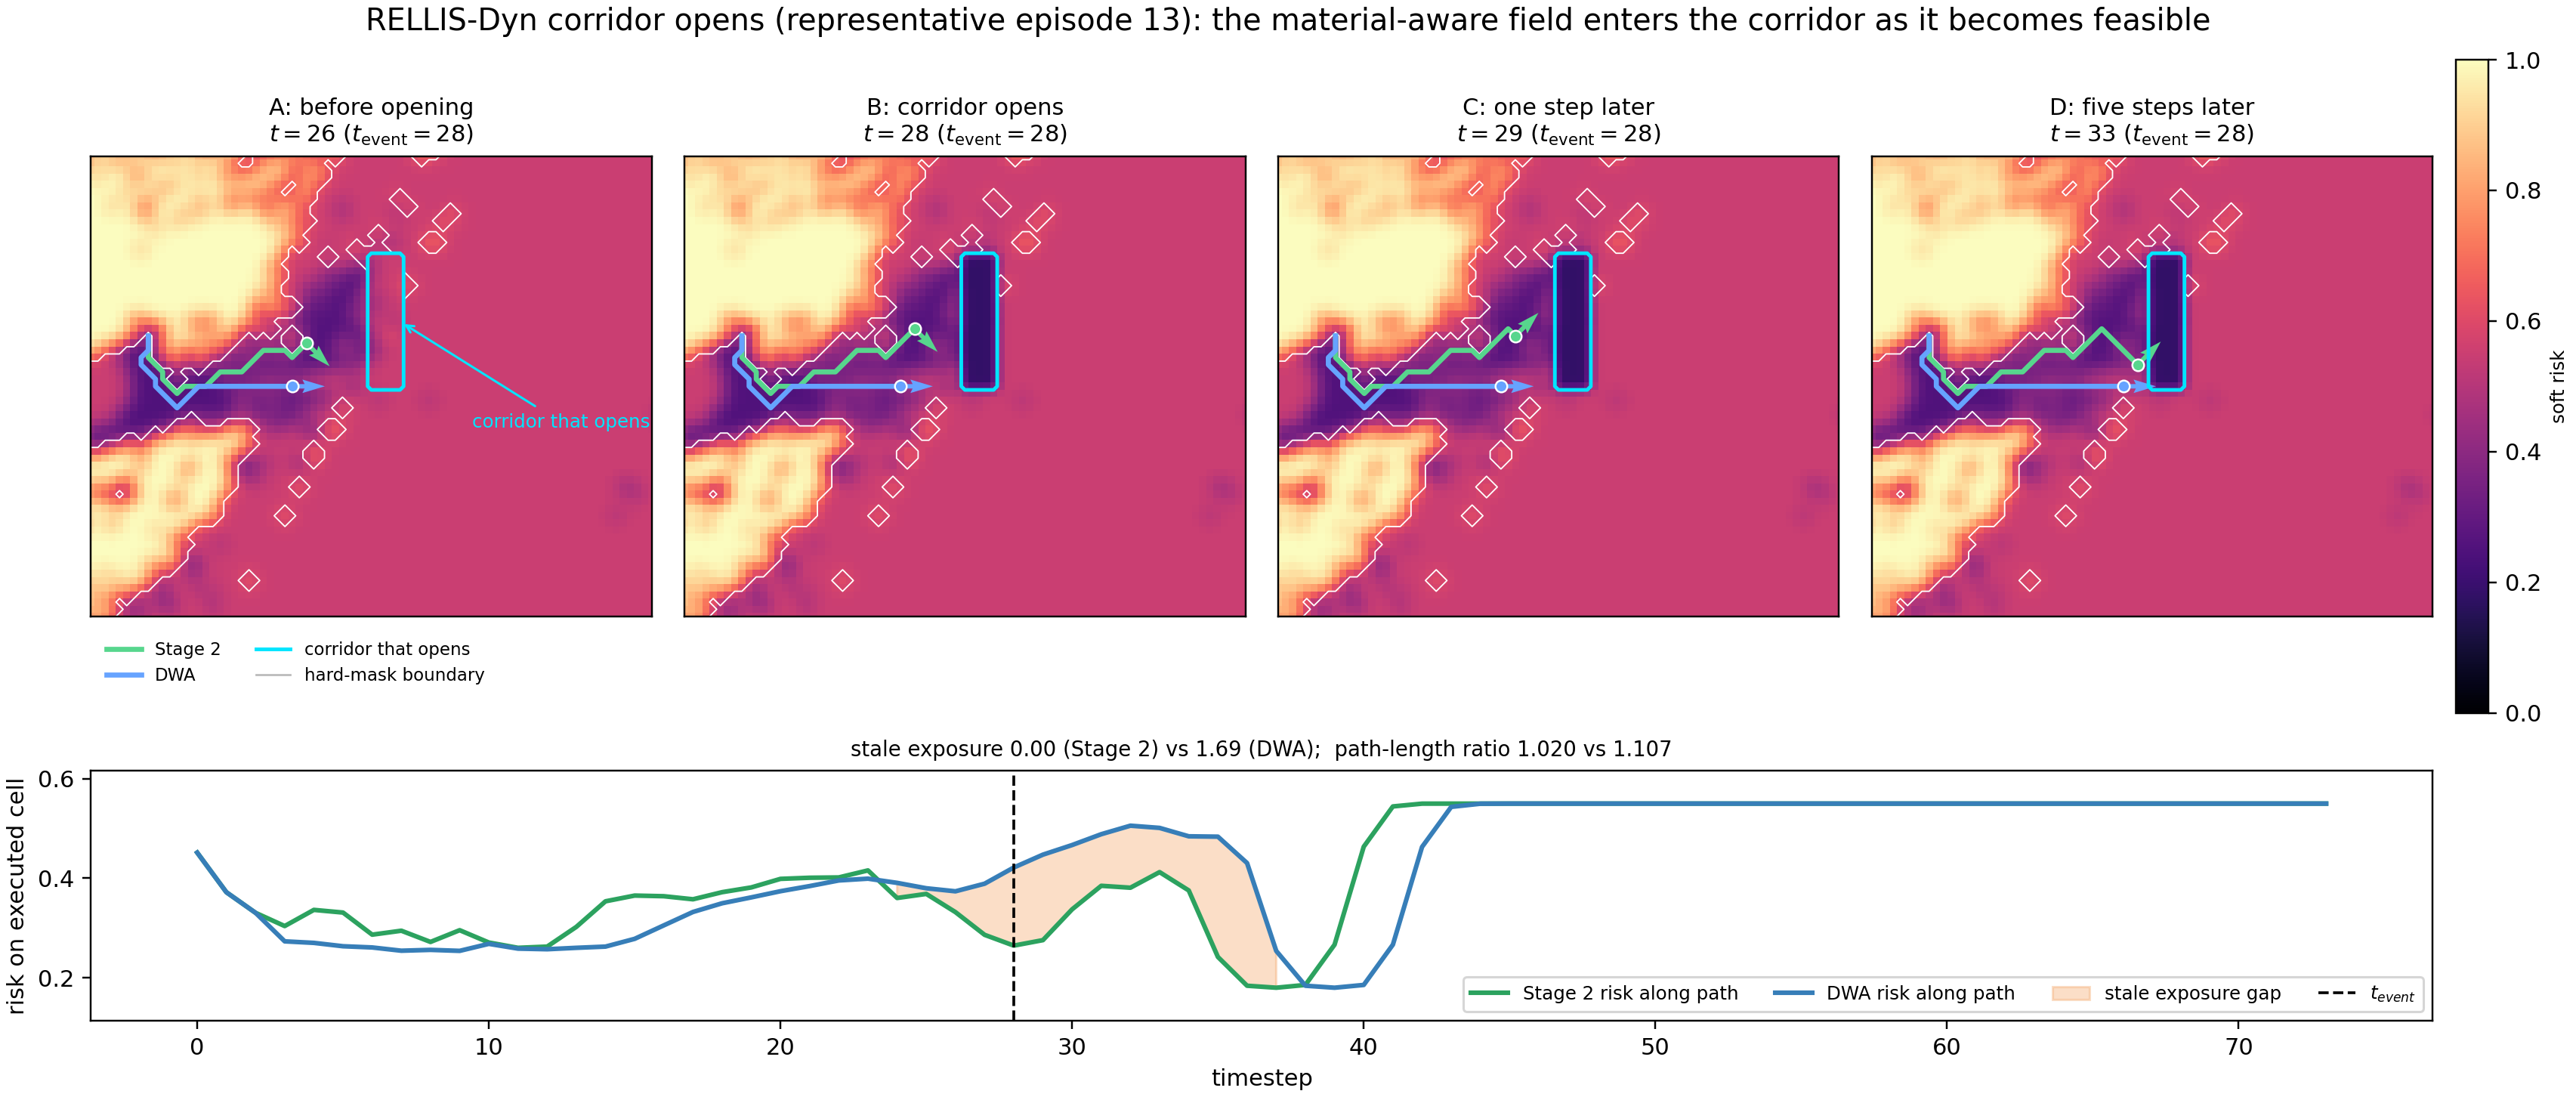
\includegraphics[width=\textwidth]{figures/rellis_dyn_corridor_opens_timeline.png}
\caption{\textbf{RELLIS-Dyn corridor opens (dynamic R1).}
A blocked low-risk corridor becomes feasible at $t_{\rm event}$.
the context-enriched field immediately reshapes the context force and enters the lower-risk
route; DWA detects the opening one step later and accumulates stale
exposure (shaded). The bottom trace quantifies the stale-exposure gap
over the executed trajectory.}
\label{fig:rellis_dyn_corridor}
\end{figure*}

\paragraph{Within-episode temporal selectivity.}
Figure~\ref{fig:rellis_dyn_temporal} shows the delayed-required-escape
mechanism for two variants.
Route-aware CVaR keeps lateral force near zero throughout the suppression
window and activates within two steps of $t_{\rm escape}$.
The expected-cost variant activates earlier (false pre-activation $0.370$
vs.\ $0.180$), confirming that the improvement comes from CVaR's
concentration of gradient on tail rollouts.

\begin{figure*}[t]
\centering
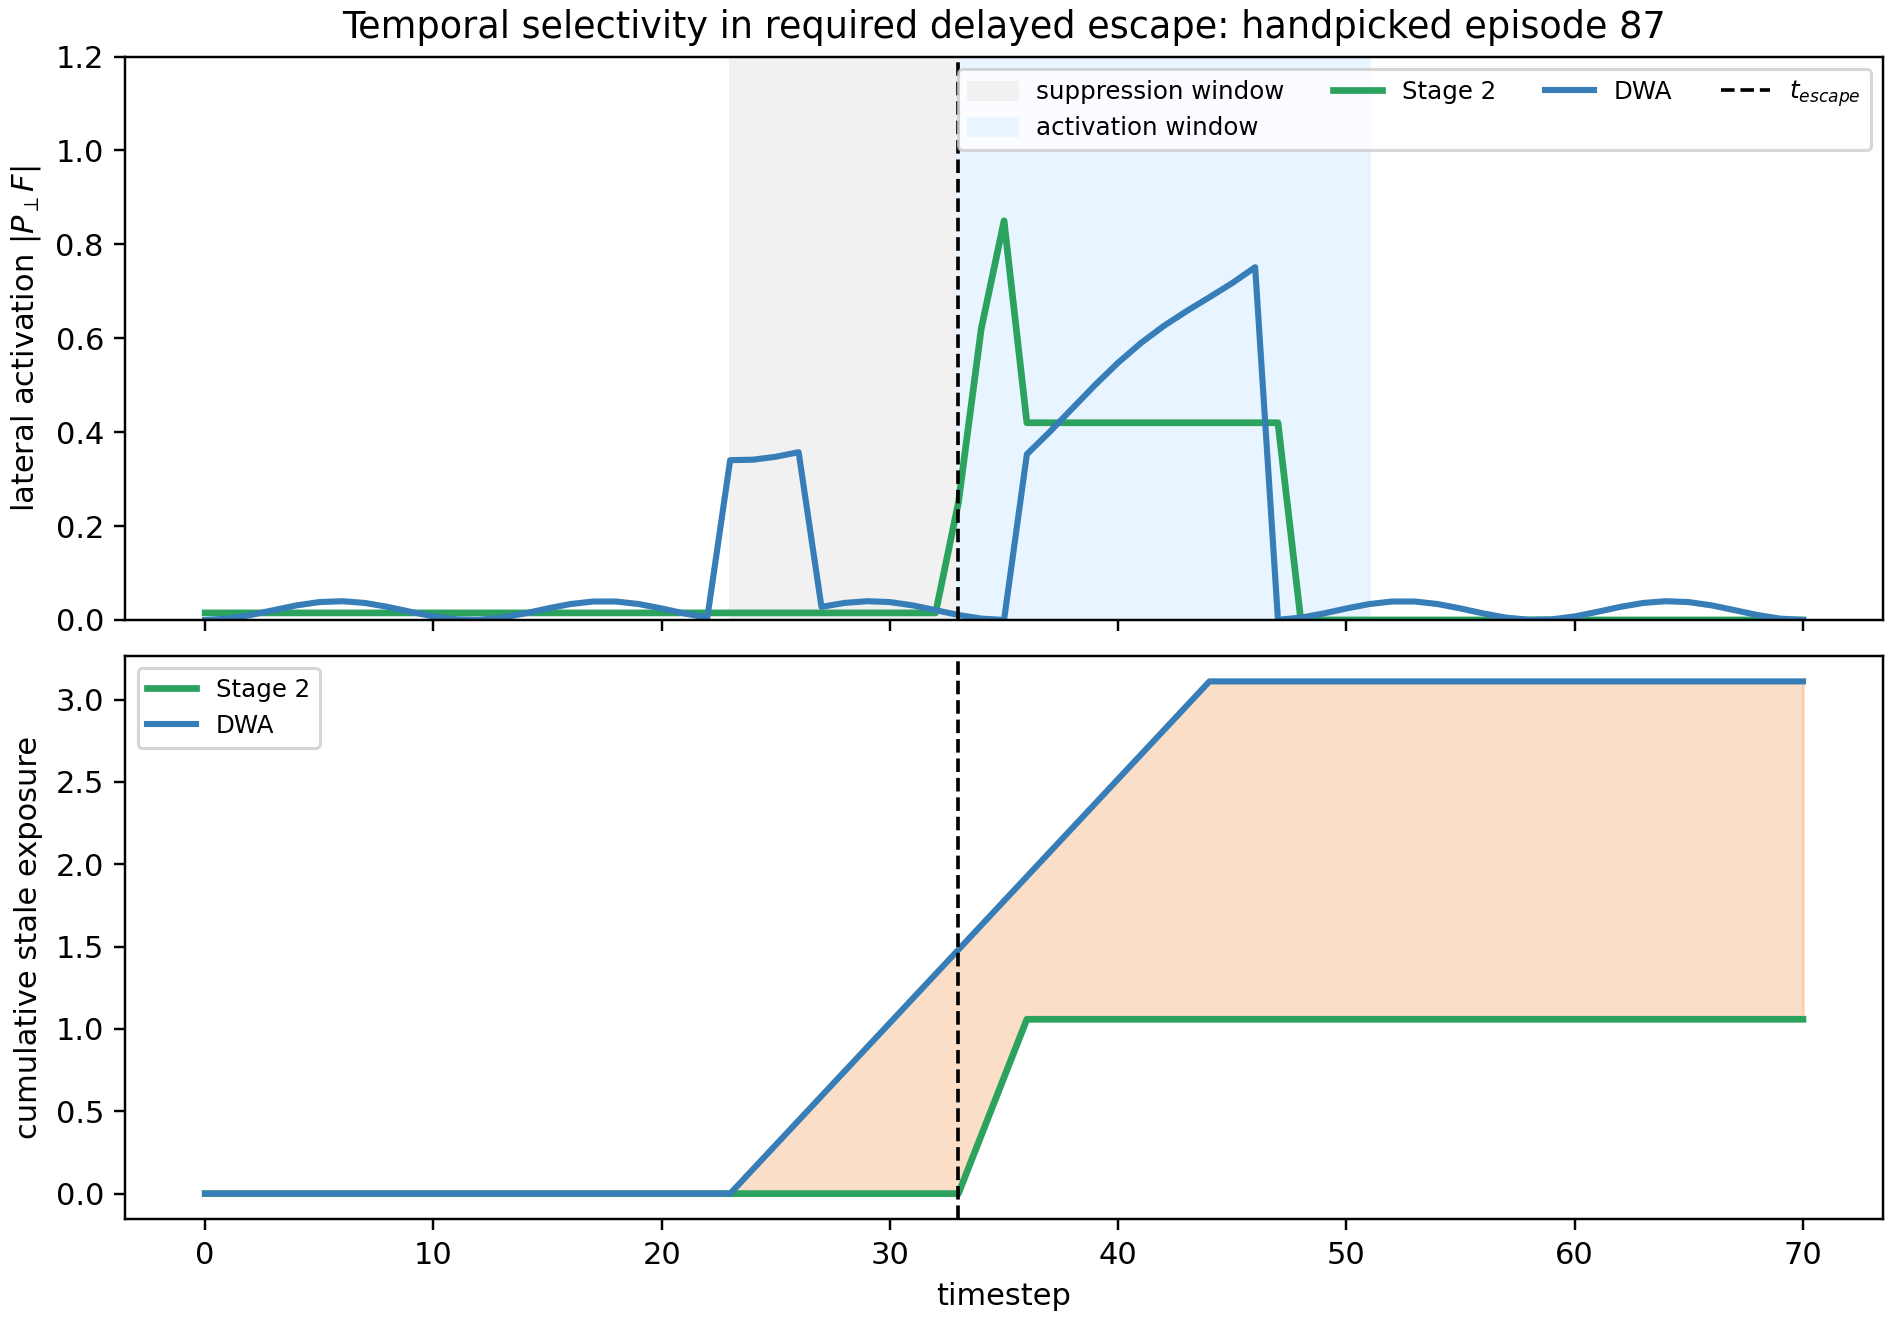
\includegraphics[width=0.75\textwidth]{figures/rellis_dyn_delayed_escape_temporal_selectivity.png}
\caption{\textbf{Within-episode temporal selectivity.}
The escape is infeasible before $t_{\rm escape}$ (gray window) and
necessary afterward.
The route-aware context-enriched field (CVaR) suppresses lateral activation during the
blocked window and activates after; false pre-activation rate
$0.180$.
The expected-cost variant activates earlier (false pre-activation
$0.370$), illustrating the contribution of tail-risk training.
DWA false pre-activates on $95\%$ of episodes, typically
$3$--$5$ steps before $t_{\rm escape}$, because partial boundary
changes trigger its reactive response before the escape is fully
open.}
\label{fig:rellis_dyn_temporal}
\label{fig:rellis_dyn_temporal}
\end{figure*}

% ----------------------------------------------------------------------
\subsection{DFC2018: Scaffold Repair}
\label{sec:exp_dfc}
% ----------------------------------------------------------------------

DFC2018 tests whether enrichment repairs a geometry-only scaffold on
a static semantic material map.
Relative to geometry scaffold, context-enriched field improves success from $0.867$ to $1.000$,
reduces catastrophic failure from $0.600$ to $0.100$, reduces
hard-hazard traversal by $96.9\%$, reduces cumulative risk by $59.2\%$,
and reduces oscillation by $90.7\%$ while keeping nearly the same
path-length ratio (Table~\ref{tab:dfc_geom_ctx}).
The full planner comparison is in Appendix~\ref{app:dfc_full};
full-map planners with global access obtain lower raw static risk
but context-enriched field repairs the learned scaffold with smoother continuous
trajectories and no oscillation.

\begin{table}[t]
\centering
\caption{\textbf{DFC2018 geometry-to-context outcome shift.}
Means over $30$ paired test episodes.
The context-enriched field reduces severe exposure without buying lower risk through a large
detour.}
\label{tab:dfc_geom_ctx}
\scriptsize
\setlength{\tabcolsep}{3pt}
\renewcommand{\arraystretch}{1.08}
\resizebox{\linewidth}{!}{%
\begin{tabular}{lrrrrrr}
\toprule
Method & Success$\uparrow$ & Cat.\ fail$\downarrow$ & Hard len.$\downarrow$
       & Risk$\downarrow$ & Len.\ ratio & Osc.$\downarrow$ \\
\midrule
Geom. scaffold    & $0.867$ & $0.600$ & $21.106$ & $23.267$ & $1.044$ & $82.212$ \\
\textbf{Ctx-enriched}    & $\mathbf{1.000}$ & $\mathbf{0.100}$ & $\mathbf{0.658}$
                    & $\mathbf{9.493}$ & $1.045$ & $\mathbf{7.629}$ \\
\bottomrule
\end{tabular}}
\end{table}

% ----------------------------------------------------------------------
\subsection{Highway-env: Interaction Selectivity}
\label{sec:exp_highway}
% ----------------------------------------------------------------------

Highway-env tests the same R1/R2 split under dynamic interaction risk.
The open slow-leader scenario is the interaction analog of corridor
opens: a feasible adjacent lane improves TTC, so the lateral channel
should activate.
The boxed slow-leader scenario is the interaction analog of
moving-obstacle-blocks-detour: the escape is infeasible, so the channel
should be suppressed.

Table~\ref{tab:highway_mechanism} shows the mechanism ablation
(RQ1/RQ2 in the interaction domain).
Removing the lateral context channel causes the agent to collide with
the slow leader on every episode; adding it without the TTC/dynamic-risk
channel causes off-road failure in the boxed scenario.
Only the full context-enriched field system correctly passes the open leader and
suppresses the maneuver when boxed.
MOBIL-IDM and risk-aware MPC outperform context-enriched field overall (Appendix
Table~\ref{tab:app_highway_baselines}); the context-enriched field is the strongest
\emph{learned} method in this suite and is the only one exhibiting
the intended activation/suppression mechanism.

\begin{table}[t]
\centering
\caption{\textbf{Highway mechanism ablation} ($200$ paired seeds per
scenario).
The lateral channel enables passing; the TTC/dynamic-risk channel
suppresses the same maneuver when boxed.
Full scenario-level results in Appendix
Table~\ref{tab:app_highway_baselines}.}
\label{tab:highway_mechanism}
\scriptsize
\setlength{\tabcolsep}{3pt}
\renewcommand{\arraystretch}{1.08}
\resizebox{\linewidth}{!}{%
\begin{tabular}{lrrrrrr}
\toprule
Variant & Def.\ off-road$\downarrow$ & Slow coll.$\downarrow$
        & Slow succ.$\uparrow$ & Boxed coll.$\downarrow$
        & Boxed off-rd.$\downarrow$ & Boxed spd.$\uparrow$ \\
\midrule
No lateral context           & $0.00$ & $1.00$ & $0.00$
                             & $1.00$ & $0.00$ & $22.33$ \\
Lateral context only         & $0.20$ & $0.00$ & $1.00$
                             & $1.00$ & $0.00$ & $22.33$ \\
\textbf{Lateral + TTC/dyn.\ risk} & $\mathbf{0.00}$ & $\mathbf{0.00}$
                             & $\mathbf{1.00}$ & $\mathbf{0.00}$
                             & $\mathbf{0.00}$ & $\mathbf{7.57}$ \\
\bottomrule
\end{tabular}}
\end{table}

% ----------------------------------------------------------------------
\subsection{Ablations and Interpretation}
\label{sec:exp_interpretation}
% ----------------------------------------------------------------------

\paragraph{Three contributions, three paired comparisons.}
Table~\ref{tab:delayed_escape} isolates the contributions cleanly.
\emph{Hamiltonian structure} (black-box CVaR vs.\ route-aware CVaR):
same objective, different architecture; navigation success $0.200$
vs.\ $0.810$.
The black-box pattern-matches risk gradients statically but cannot
translate that into temporal suppression at execution time.
\emph{CVaR training} (expected cost vs.\ route-aware CVaR):
same architecture, different objective; false pre-activation $0.370$
vs.\ $0.180$, navigation success $0.620$ vs.\ $0.810$, violation
CVaR $0.855$ vs.\ $0.740$.
CVaR concentrates gradient on the tail rollouts where the force channel
must act at the right moment.
\emph{Context-conditioning} (fixed-coeff vs.\ route-aware CVaR):
same architecture and objective, fixed vs.\ predicted $\lambda_s,\lambda_h$;
navigation success $0.030$ vs.\ $0.810$.
Without the CNN head, the method cannot modulate force magnitude with
context and suppresses nothing.

\paragraph{Force channel vs.\ loss reweighting (RQ6).}
Across DFC and RELLIS-Dyn, risk-loss-only reduces neither hard-hazard
exposure nor temporal lag reliably.
In RELLIS-Dyn, risk-loss-only hard exposure is $[FILL]$ vs.\ context-enriched field
$[FILL]$; in DFC, catastrophic failures drop from $0.60$ to $0.10$
only with context-enriched field.
The risk signal must enter the Hamiltonian force channel rather than
remain in the scalar training objective.

\paragraph{Reactive, planning, and Hamiltonian methods occupy different
tradeoff positions.}
Reactive baselines (DWA, CBF-QP) handle hard-boundary avoidance events
well but false pre-activate on discovery events (false pre-activation
$0.950$ for DWA on delayed escape).
Planning baselines reduce violation when given replan budget but pay
$9$--$68\times$ more replans.
The route-aware context-enriched field occupies the zero-replan, gradient-following
position: strongest on soft-risk and escape-discovery events, weaker
on moving-obstacle events where reactive boundary following is
sufficient and gradient following offers no advantage.
The eight-event group Pareto in Appendix
Figure~\ref{fig:app_rellis_dyn_pareto} shows each method's position
on reaction delay vs.\ post-event violation CVaR.

\paragraph{Limitations.}
Several limitations bound the current results.
First, the soft-hazard barrier $b_{\mathrm{sp}}(\phi)$ is a
differentiable repulsive term, not a formal CBF certificate; we claim
empirical violation reduction and tail-risk improvement, not forward
invariance (Appendix~\ref{app:theory}, Sec.\ A.9).
Second, performance depends on the quality of the local risk map: the
RELLIS main experiment uses oracle semantic labels, and the perception
robustness table (Appendix Table~\ref{tab:app_rellis_perception})
shows moderate degradation under label corruption.
Third, the route-aware gate samples $K$ local candidate rollouts at
each step; on hardware with tight latency budgets, gate overhead
must be profiled (reported in the ms/step column of
Table~\ref{tab:rellis_dyn_agg}).
Fourth, DWA and MOBIL-IDM remain stronger on moving-obstacle avoidance
and full highway control respectively; the method's advantage is
specific to local gradient-following for material and interaction
risk.

\clearpage
